\chapter{Data Mining in Nearby Galaxies}
\label{ch: paper3}
%----------------------------------------------------------------------------------------
%----------------------------------------------------------------------------------------
%----------------------------------------------------------------------------------------
%Intro
%----------------------------------------------------------------------------------------
%----------------------------------------------------------------------------------------
%----------------------------------------------------------------------------------------
\section{Introduction} 
% Nearby galaxies and their importance 
Nearby galaxies play an important role in our understanding of galaxies' formation and evolution.
Nearby galaxies are defined as those close enough that we are able to observe their structure and composition in detail.
As a result, many studies have been devoted to finding relations between physical properties of galaxies, such as morphology, star formation rate (SFR), stellar mass, metallicity, and amount of gas, both for spatially-resolved regions and galaxies as a whole~\citep[e.g.][]{Wong13,Leroy08}, and many others use these results in analyzing observations of high-redshift galaxies~\citep[e.g.][]{Freundlich13,Walch11}.
%Advances in technology allow us to collect data from the sky. %PB - commented out
Surveys such as KINGFISH~\citep{Kennicutt11} and THINGS~\citep{Walter08} have made observations of nearby galaxies in various wavelengths and from these data we can measure physical properties such as stellar mass, star formation rate (SFR), dust mass, and gas mass~\citep[e.g.][]{Eskew12,Dale09,Calzetti07}.

% A little bit about M31 and previous studies in M31.
The Andromeda galaxy (M31), at a distance of $\sim$~0.78~Mpc, is the closest spiral galaxy to the Milky Way~\citep{McConnachie05}.
Images of this galaxy provide us with a detailed view of the inside of a spiral galaxy as seen from an external perspective.
M31 has been observed by many telescopes including the {\textit Hubble}, \Spitzer and \Herschel space telescope.
\cite{Barmby06} used data from the \Spitzer Infrared Array Camera \citep[IRAC;][]{Fazio04} to show the spatial distribution of Polycyclic Aromatic Hydrocarbons (PAHs) in the interstellar medium (ISM) of M31.
Using data from the Multiband Imaging Photometer for Spitzer (MIPS) instrument, \cite{Gordon06} studied the morphology of M31's dust.
\cite{Azimlu11} and \cite{Sanders12} catalogued and studied \hii~regions of M31.
\cite{Draine14, Mattsson14, Viaene14, Smith12} and~\cite{Fritz12} used \Herschel data to study dust in the ISM of the galaxy.
Properties of the current stars in the galaxy were studied by many groups~\citep[e.g.][and references therein]{Tamm12,Dalcanton12,Massey07}.
\cite{Rahmani16, Ford13} and \cite{Tabatabaei10} measured the spatially-resolved SFR in M31 in order to study star formation laws, and~\cite{Dim15} and \cite{Kapala15} used infrared spectroscopy to study PAHs and atomic and molecular line emission in the ISM.

Although all these studies measured some properties of M31, or answered specific scientific questions about this galaxy, we still do not have a complete picture of underlying processes in the galaxy.
What is the correlation between PAHs and SFR, dust mass, and gas mass in M31? 
Are PAH features in M31 similar or they can be divided into various groups? If so, what are the properties of each group?
Does the intensity of PAH emission depend on the underlying structure of their position? %PB: I don't understand what you mean by "underlying structure of their position"
How do they compare to properties of galaxies? %PB: what is "they"
The properties of M31 that derived in various studies and observational data of this galaxy can be used for a knowledge discovery and data mining study.
%The amount of data for M31 makes this galaxy a suitable target for a knowledge discovery and data mining study.
The Pinwheel Galaxy (M101), with distance of 6.7~Mpc~\citep{Freedman01}, is another nearby galaxy that has been well-observed and studied~\citep[e.g. ][and references therein]{Kennicutt11,Dale09, Leroy08, Gordon08}.
M101 is a large spiral galaxy with several \hii~regions and a large metallicity gradient from centre to outskirts~\citep{Kennicutt03}.
In case of dimensionality data from M101 is a suitable addition to M31 data for a data mining study. %PB: don't understand "In case of dimensionality"
Knowledge discovery and data mining methods are designed to extract hidden information from data and have been tested in many astronomical studies~\citep[e.g.][and references therein]{Ball10}.
However, this study is the first to use a data mining method on observations of nearby galaxies.

% data mining and clustering in general; when we have so many data and we want to map them
\cite{Ball10} gave an extensive review of data mining and machine learning algorithms and their usage in astronomy.
A data mining algorithm learns about data from training, which can be supervised or unsupervised.
Supervised training refers to methods that use examples of the desired output to learn about input data; these are valuable tools for classifying data with known target values.
Unsupervised methods train without any prior knowledge of output results: 
they work solely based on the underlying structure of the input data.   
The unsupervised methods are very useful tools in knowledge discovery studies, where we have limited pre-expectations for the data or when we want to make sure that we did not miss any valuable information in previous studies.

The purpose of the present work is to use M31 observations to generate new insights into nearby galaxies, with a focus on relations between PAHs and other properties of the galaxy.
There are very few studies on relations between properties of M31 with its PAH features. %generate?!
\cite{Cesarsky98} studied PAH spectra observed by ISOCAM spectro-imaging in four regions in M31 and found that PAH features in M31 differ from those in other galaxies in having weak or no $6.2 - 8.6$~$\mu$m emission with enhanced 11.2~$\mu$m emission. 
However,~\cite{Dim15} using {\it Spitzer}/Infrared Spectrograph~\citep[IRS;][]{Houck04b} observations, found that the PAH spectra of M31 have the same features as the spectra of other nearby star-forming galaxies.
Those authors re-evaluated the ISOCAM data to compare them to IRS data and found that the earlier results were likely due to incorrect background subtraction. %(PB), but the results were inconclusive. %%%%% !!!!!%%%%
Using IRAC imaging observations,~\cite{Barmby06} found good agreement between the M31 SFR derived using observed 8~$\mu$m luminosity with other 
star formation indicators such as \halpha and far infrared luminosity.
\cite{Draine14} found that the PAH abundance in M31 is almost constant up to a galactocentric radius of $\sim 20$~kpc.
With data mining techniques we address the question of whether,
compared to other galaxies, PAH features in M31 are unique as~\cite{Cesarsky98} claimed, or  are normal as ~\cite{Dim15} and \cite{Draine14} concluded.


%this project 1 M31 and its extensive data we do not have any SOM in nearby galaxies
In this project we apply the self-organizing map algorithm (SOM) to M31 data, training 1D and 2D networks.
Using networks with fewer neurons, we study the properties of the clusters and investigate relations between PAH features and other quantities in M31.
We create 2D SOMs from subsets of the data as well as all available data, which helps us to understand the effect of each input on the position of the clusters in the SOM.
We apply the 2D trained networks to the M101 data to check whether it has similar properties.
If our hypothesis is correct, we should be able to see that regions in M31 and M101 with the same positions in the SOM have the same properties.


We describe the SOM method in Section $\S$~\ref{sec: method}. %PB: I think you use either "Section" or $\S$, not both.
In Section $\S$~\ref{Sec: data_SOMN}, we present the observational data from M31 and M101 that we use in this study.
The results of the 1D SOM networks and the study of PAHs in M31 are presented in Section $\S$~\ref{Sec: 1d_cluster}.
In Section $\S$~\ref{sec: 2d_cluster}, we present the results of 2D SOM networks and their use in extracting information about other galaxies.
In Section $\S$~\ref{sec: summary}, we summarize our results and discuss potential future work in this subject.

%----------------------------------------------------------------------------------------
%----------------------------------------------------------------------------------------
%----------------------------------------------------------------------------------------
%Method
%----------------------------------------------------------------------------------------
%----------------------------------------------------------------------------------------
%----------------------------------------------------------------------------------------

\section{METHOD}
\label{sec: method}
\subsection{Choosing an Algorithm}

Some of the most tested methods of data mining in astronomy are artificial neural networks (ANNs)~\citep[e.g.][and references therein]{Hossein14,Hossein16}.
ANNs are designed to work in the same way that the neurons work in a human brain.
These are networks of interconnected neurons (nodes), in which all of the connections are weighted.
These networks are used to study nonlinear and complex relations between input and output data.
One of the most well-known unsupervised neural networks in astronomy is a Kohonen self-organizing map (also called self-organizing map, or SOM).
SOMs visualize complex data~\citep{Kohonen82} and show simple geometrical relationships in non-linear high dimensional data~\citep{Kohonen98}.
The result of a SOM is a 1D or 2D network of neurons, which shows the positions of clusters and their relative distance.
Since the 1990s, many studies have utilized SOMs for object classification and clustering (e.g. classifying quasars' spectra, star/galaxy classifications, gamma-ray burst clustering and light curve classification) and photometric redshift estimation~\citep[e.g.][]{Odewahn92, Hernandez94, Murtagh95, Maehoenen95,Scaringi09,Geach12,Fustes13,Meusinger16,Rahmani16b}. %%% Why I cannot add submitted in front of the high-z paper %PB: MNRAS style guide says "Private communications or papers in preparation should be listed as such in the text, but omitted from the reference list, e.g. Smith (in preparation) shows that… " -- but I'm not clear on whether this applied to submitted papers or not

The K-means algorithm, SOMs, and hierarchical clustering are the main unsupervised methods that are used in astronomical studies~\citep[e.g.][]{DAbrusco12, Aycha16}. %%add one or two more
For both K-means and SOM algorithms, the user must define the number of clusters, and the algorithms decide how to separate the data into the desired number of clusters.
In the hierarchical clustering method, the user must define dissimilarity between the groups; the algorithm combines (or divides) existing groups based on their dissimilarity and creates a hierarchical structure. 
Comparing the SOMs, K-means and hierarchical clustering methods shows that in some cases the hierarchical clustering method mis-classifies the data~\citep[][and references therein]{Mangiameli96}.
We chose the SOM method over the K-means method due to the fact that SOMs not only cluster data, but also show similarities and dissimilarities between the clusters.
Therefore, we can cluster our sample data and study the underlying structure simultaneously.

 \subsection{Self Organizing Maps}
 \label{sec: som}
 The SOM is a clustering method which reduces the dimensionality of data, while preserving topological features~\citep{Kohonen98}. 
 The results of the SOM are shown with a map of neurons, which their numbers are set by the user.
 Each neuron has a fixed position in the map and may contain one or more samples from the input data,~\boldit{V} $\in \Re^n$. % Els said the simbols should be describe?! I think it is pretty obvious! %PB: most are pretty obvious, but mention what $n$ is here
 A weight vector,~\boldit{W} $\in \Re^n$, with the same dimension as the input data, is associated with each node and will be varied during the training process.
 The process of creating an SOM happens over a series of $N$ iterations.
 In each iteration, the algorithm calculates the Euclidean distance for each node $j$ as $D_j^2= \sum_{i=0}^{i=n} (V_i - W_i)^2$, and finds a neuron with $D_{j_,{\mathrm min}}$. 
 This neuron is the winner node and is calling Best Matching Unit (BMU). 
 The weight vectors in the neighbourhood of the BMU will change according to the Kohonen learning rule (equation~\ref{equ: weight adj}). 
  \begin{equation}
            \label{equ: weight adj}
            W(t+1)=W(t)+L(t) \times R(t) \times(V(t)-W(t))
 \end{equation}
where $L(t) = L_0 e^{(-t/\tau)}$ is the learning factor, which prevents the divergence of the SOM, and $R(t)=\exp(-\frac{D_j^2}{2r^t_{BMU}})$ is the influence rate, which determines how the weight of each node will change. %PB: mention what L_0, \tau, r are
Values for the number of neurons, $L(t)$ and $R(t)$ are arbitrary. 
~\cite{Geach12} and \cite{Rahmani16b} demonstrate the algorithm of the SOM in more detail.


     In order to create self-organizing maps, we used the \textsc{matlab} neural network toolbox~\citep[NNT,][]{matlabtolbox}.
     An SOM in \textsc{nnt} can be created by the \textsc{newsom} library, which works in two phases, the ``ordering phase" and ``tuning phase" . 
     Phase one is the ``ordering phase". 
     This phase starts with maximum neighbourhood distance, and an initial high learning factor, usually 0.9, which is provided by the user. 
     The ordering phase continues for the requested number of iterations.
     At the end of the iterations, the learning factor reduces to the tuning phase learning factor and the neighbourhood distance reaches the value set by the user. 
     The second phase is the ``tuning phase".
     In this phase the neighbourhood distance is at its minimum, but the learning factor decreases very slowly.
     This minimum neighbourhood distance and slowly decreasing learning factor helps to fine tune the topology results and causes a more stable SOM. 
     The number of iterations in this tuning phase must be much greater than the number of iterations in ordering phase, to allow the tuning to happen slowly. 
     We chose the number of epochs in the tuning phase to be 3 times more than the number of epochs in the ordering phase.
     
     To present our results, we use \textsc{nnt}'s built-in plotting tool.
     Specifically, we combine two of the plots in this tool: a hits map, which shows the number of times each neuron has become the winner (hits), and a distance map, which shows the distance between weight vectors of those neurons.
     In the maps, the purple hexagonal shapes show the neurons. 
     The distances are shown by the grey-scale colours: the darker the colour, the larger the distance between neurons.
     Neurons with zero hits are left empty.
     In Section~\ref{sec: mock_sample} we used \textsc{newsom} to create SOMs from a mock sample to illustrate how this method works and how to interpret the results.

     One feature of the SOM method is that there is no rule or restriction on the number of clusters.
     Users must decide the size of the network based on their data set and their usage of the results.
     There has been a few attempts to find a rule for restricting the number of neurons based on the input sample \citep[e.g.][]{Vesanto05}, but none of them are certain. 
     We varied the size of SOMs from $1\times2$ to $50\times50$ in order to choose the most suitable size for the maps we generated, and found that based on the size of our sample, the best size for the 2D SOMs was $10\times10$. 
     We created our final SOMs with initial values for number of iterations in ordering phase, ordering phase learning factor, tuning phase learning factor, and tuning phase neighbourhood distance of 500, 0.9, 0.02, and 1, respectively. 
     %Also for each grid we created different SOM with different, learning factors, neighbourhood distances, and iteration numbers to find the optimize result for our sample.
     %Based on our data we created our final SOMs with following initial values: number of iteration in ordering phase = 1000; ordering phase learning factor = 0.9; tuning phase learning factor= 0.02; and tuning phase neighbourhood distance to be 1.
     %All the other parameters are default values in \textsc{ newsom} library and cannot be changed by the users. 
     
    
\subsection{Mock sample}
\label{sec: mock_sample}
 
         \begin{figure}
                \centering
                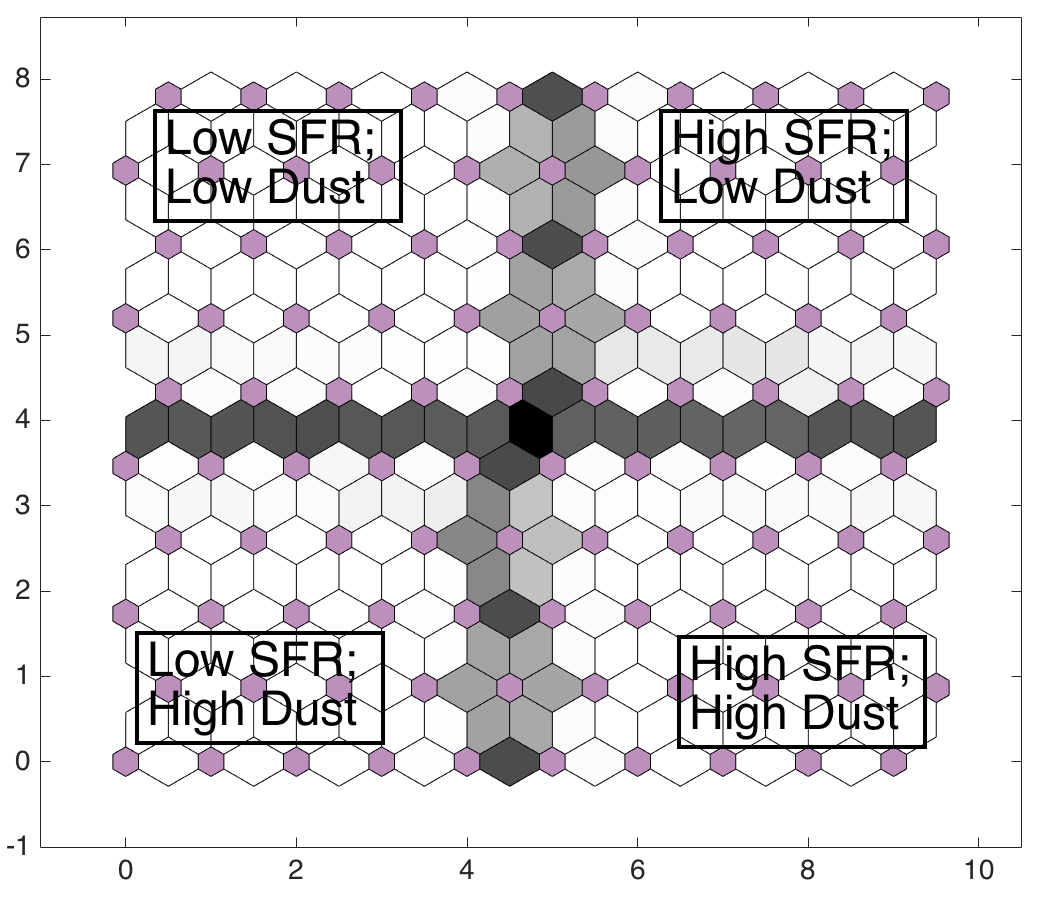
\includegraphics[width=0.5\textwidth]{../image_paper3/images0.01/mock_sample.png}
            \caption{SOM of the mock sample. The axes show the position of the neurons. Hexagonal shapes represent the neurons. The grey-scale colours show the differences between neuron weights, where white is the minimum difference and black is the maximum one.}
            \label{fig: sample}
        \end{figure}
 
To show how self-organizing maps work, we created a mock sample containing only a few regions.
Each sample had two properties: the amount of dust and the star formation rate, where the possible values were
either 0 or 1 for low or high SFR, and 0 or 0.5 for a low or high amount of dust. 
 We generated an SOM from the sample with a size of $10 \times 10$, using the method described in Sec.~\ref{sec: som}.
 Fig. ~\ref{fig: sample} shows the SOM of the mock sample. 
 The axes show the position of the neurons in a $10 \times 10$ network and the hexagonal shapes are the neurons.
 
Using this method, as expected, we are able to divide the mock sample into 4 distinct groups. Their boundaries are shown by grey colours in Fig.~\ref{fig: sample}: regions with high SFR and high dust content, regions with low SFR and high dust content, regions with high SFR and low dust content, and regions with low SFR and dust content. 
%The plot in the Fig.~\ref{fig: sample} clearly shows these divisions.%PB: commented out.
In Fig.~\ref{fig: sample}, the upper part belongs to regions with low dust content, while the lower part belongs to regions with high dust content.
The left part of the plot is where regions with low SFR belong and the right side is for high SFR regions.
Grey to black colours show the border between regions.
This network is considered to be a trained network, and can be used to cluster any new data set with similar entries.

Having two regions with exactly the same values in all their quantities with real data is extremely unlikely. 
If, in an input data set, there are two entries with similar (but not identical) values in all dimensions, one can find a network that separates these two entries in two groups.  
However, in case of multiple similar entries in a dataset, the number of neurons must be much higher than the number of entries for complete separation.
Therefore, the user learns about similarity or dissimilarity of members of the input dataset based on the ratio of the number of entries in the dataset and  the number of neurons. 

%----------------------------------------------------------------------------------------
%----------------------------------------------------------------------------------------
%----------------------------------------------------------------------------------------
%DATA
%----------------------------------------------------------------------------------------
%----------------------------------------------------------------------------------------
%----------------------------------------------------------------------------------------

\section{Study sample} %%or sample study?! %PB: study sample is OK
\label{Sec: data_SOMN}

Our study includes 10 regions in M31 (Fig.~\ref{fig: regions in m31}) and 8 regions in M101 (Fig.~\ref{fig: regions in m101}). 
These specific regions were chosen for the availability of \Spitzer/IRS 5--15$\mu$m  spectroscopy covering the PAH emission bands.
Besides PAH band strengths, for each galaxy, we use spectroscopic and photometric observations as well as their derived properties, such as SFR, stellar mass, dust luminosity (L$_{\rm dust}$) and mass, metallicity, and gas mass.
Table~\ref{tab: data} shows the full list of data for both M31 and M101.
All data were divided by the area of their region (in arcsec$^2$), to remove the distance factor from the data and compare values across galaxies.
Since the spatial resolution of the observations varies from $<1$\arcsec to 60\arcsec $\times$ 90 \arcsec, any attempt to match resolution would have caused a loss of information in some of the input quantities (e.g. the spectroscopic data).
In this project we used flux per unit area, which the convolution methods conserve~\citep{Aniano12}, as the input data.
Therefore, we did not perform any resolution matching and used data at their original resolution. %PB: Need to discuss these last few sentences; not sure I understand what you're saying.


\import{../image_paper3/text_files/tables/}{tab_data.tex}

\begin{figure}
  \begin{subfigure}[b]{0.5\textwidth}
        \centering
    %\centering
        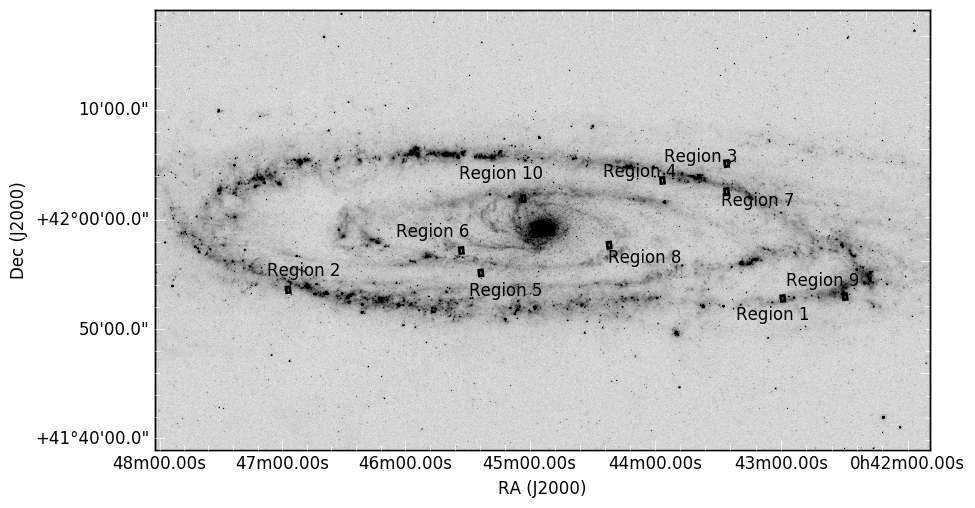
\includegraphics[width=0.97\textwidth]{../image_paper3/images0.01/M31/M31.png}
        \caption{MIPS~24 $\mu$m image of M31, with positions of 10 regions studied.}
        \label{fig: regions in m31}
    \end{subfigure}
    \hfill
    \begin{subfigure}[b]{0.5\textwidth}
        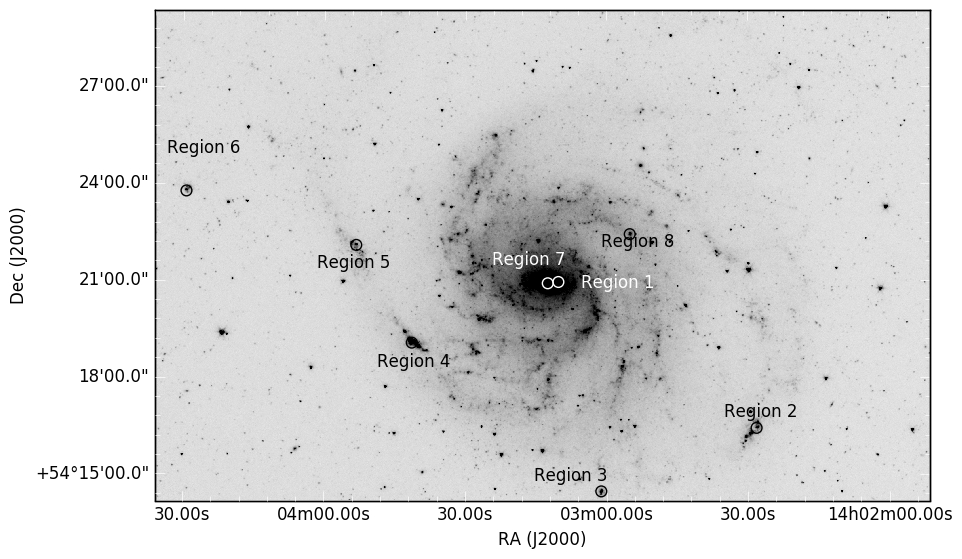
\includegraphics[width=\textwidth]{../image_paper3/images0.01/M101/M101.png}
        \caption{IRAC 3.6 $\mu$m image of M101, with positions of  8 regions studied.}
    \label{fig: regions in m101}
    \end{subfigure}
    \caption{Position of the data in M31 (up) and M101 (down).}
\end{figure}

%   \begin{figure}
%     \subfloat[MIPS 24~$\mu$m image of M31~\citep{Gordon06}, with position of 10 regions from~\cite{Dim15} \label{fig: regions in m31}]{
%       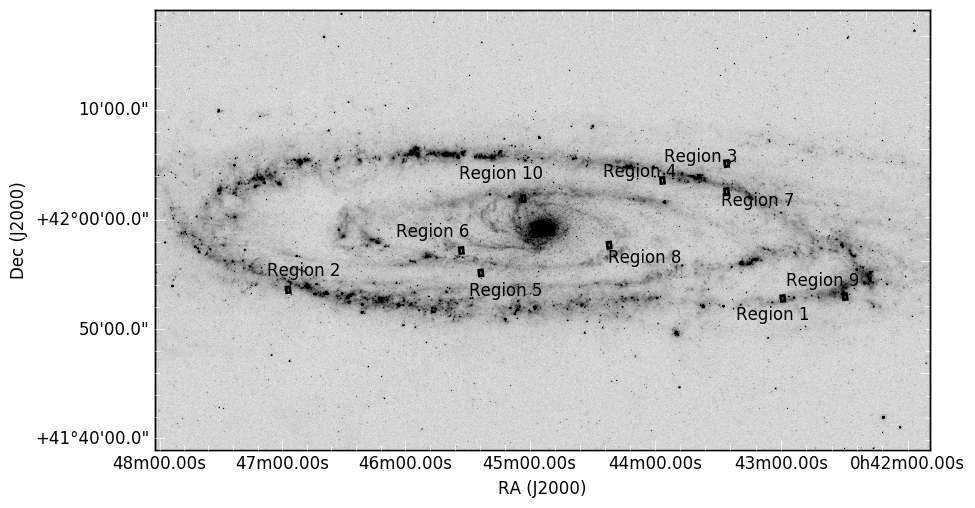
\includegraphics[width=0.5\textwidth]{../image_paper3/images0.01/M31/M31.png}
%     }
%     \hfill
%     \subfloat[IRAC 3.6~$\mu$m image of M101~\citep{Dale09}, with position of 8 regions.\label{fig: regions in m101}]{
%       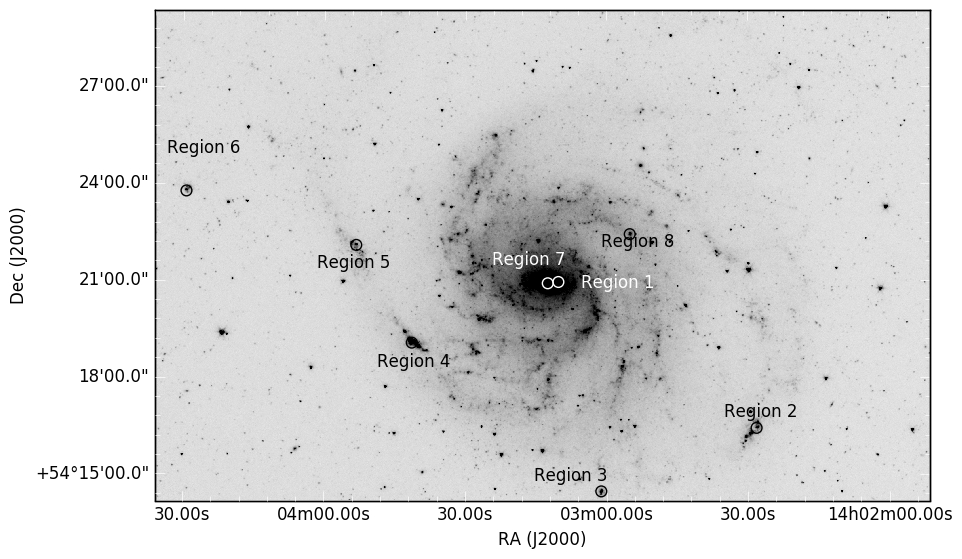
\includegraphics[width=0.5\textwidth]{../image_paper3/images0.01/M101/M101.png}}
%     \caption{Position of regions that the input data for SOM that obtained from there in M31 (up) and M101 (down).}
%     \label{fig:dummy}
%   \end{figure}

    \subsection{M31 observations}
     \label{Sec: data_M31_SOMN} 
     
     \cite{Dim15} used {\it Spitzer}/IRS observations to study PAHs in 10 regions chosen to span a range of mid-infrared flux ratios in M31 (Fig.~\ref{fig: regions in m31}). 
     Fluxes and equivalent widths of PAH and atomic line features were measured using the~\textsc{pahfit idl} tool~\citep{Smith07b}.
     \cite{Dim15} also measured metallicity and radiation hardness index (RHI) for these 10 regions.
     We used the measured PAH feature fluxes, metallicity and RHI of each region as the input for self-organizing maps.
     
    For the photometry part of the sample, we used the \GALEX \citep{Martin05} far-ultraviolet and near-ultraviolet (FUV and NUV) channel images; \halpha~(6574.7\AA), \sii~(6730.72\AA) and \oiii~(5024.9\AA) narrow band images~\citep{Massey07}, IRAC 3.6, 4.5, 5.8 and 8.0~$\mu$m images~\citep{Barmby06}; MIPS~24 and 70~$\mu$m~images~\citep{Gordon06}; and PACS 100 and 160~$\mu$m and SPIRE 250, 350, and 500~$\mu$m~\citep{Fritz12} images.
     The units of all fluxes were converted to W~m$^{-2}$ in order to be the same as the PAH fluxes.
     $^{12}$CO (J:$1\rightarrow0$) line emission images~\citep{Nieten06} and atomic gas (\hi) 21~cm emission images from~\cite{Chemin09} were added to the input data. 
     For derived values, we utilized SFR(FUV + 24$\mu$m) measured using combination of FUV and 24$\mu$m emission, stellar mass, molecular gas mass, atomic gas mass, total gas mass, and total infrared (TIR) luminosity (L$_{\mathrm TIR}$) from~\cite{Rahmani16}, and L$_{\mathrm dust}$ and dust mass from~\cite{Draine14}.
     
    \subsection{M101 observations}
    \label{Sec: data_M101_SOMN} 
    
     \cite{Gordon08} measured PAH fluxes and RHI for M101 in 8 star forming \hii~regions (Fig.~\ref{fig: regions in m101}).
     Metallicities of 6 of the 8 regions were measured by~\cite{Kennicutt03} and the other two by~\cite{Gordon08}.
     We used the NED~\footnote{The NASA/IPAC Extragalactic Database (NED) is operated by the Jet Propulsion Laboratory, California Institute of Technology, under contract with the National Aeronautics and Space Administration.} website to gather imaging observations of M101, including 
      \GALEX FUV and NUV~\citep{depaz07}, IRAC 3.6 -- 8.0~$\mu$m, MIPS~24 and 70~$\mu$m~\citep{Dale09}, and PACS~100 and 160~$\mu$m and SPIRE~250, 350, and 500~$\mu$m emission from~\cite{Kennicutt11}.
     As with M31, we used $^{12}$CO (J:$1\rightarrow0$) line emission images~\citep{Helfer03} and atomic gas (\hi) 21~cm emission images from \cite{Walter08}.
     We calculated SFR(FUV + 24$\mu$m), stellar and total gas mass maps using the same methods as for M31.
     
       \subsection{Preparing data for data mining}
    
     Correlations between some of single-wavelength emission and galaxy properties are well-known.
     Emission in the 3.6$\mu$m band traces the old stellar population very well~\citep[e.g.][]{Smith07a,Leitherer99} and it can be used to calculate the stellar mass~\citep{Eskew12}.
     FUV, \halpha, and TIR emission are indicators of star forming regions.
     In this project, we used the SFR traced by the FUV emission, corrected for foreground stars using NUV emission and for dust extinction using 24~$\mu$m emission.
     Total infrared emission is calculated from a modified version of~\cite{Draine07} calibrations using using 8, 24, 70, and 160~$\mu$m emission~\citep{Boquien10}.
    
    %To guarantee that we do not use the observed data as an input for SOM in multiple forms, we removed all the observed data that were used to calculate galaxies properties from the input sample.
    We removed all the observed data that were used to calculate galaxy properties from the input sample, to guarantee that they have not been used in multiple forms.
   % We used this new sample of observational and derived data as the main input for creating SOMs.
    To have prior knowledge of the M31 data set, %or to have an insight into the data set!
    we computed the Pearson correlation coefficients between input measurements.
    Fig.~\ref{fig: cor_all} shows the Pearson correlation coefficients with a confidence level of 95 per cent. 
    All the PAHs correlate with one another very well.
    They are also highly correlated with the SPIRE and PACS emission, L$_{\mathrm dust}$, L$_{\mathrm TIR}$, SFR and metallicity.
    The fluxes from PAHs 7.7, 8.3, 12.7 and 17~$\mu$m show a weak anti-correlation with RHI.
    In general, PAHs in our data set are highly correlated with most of the other quantities. 
    
      \begin{figure*}
                \centering
                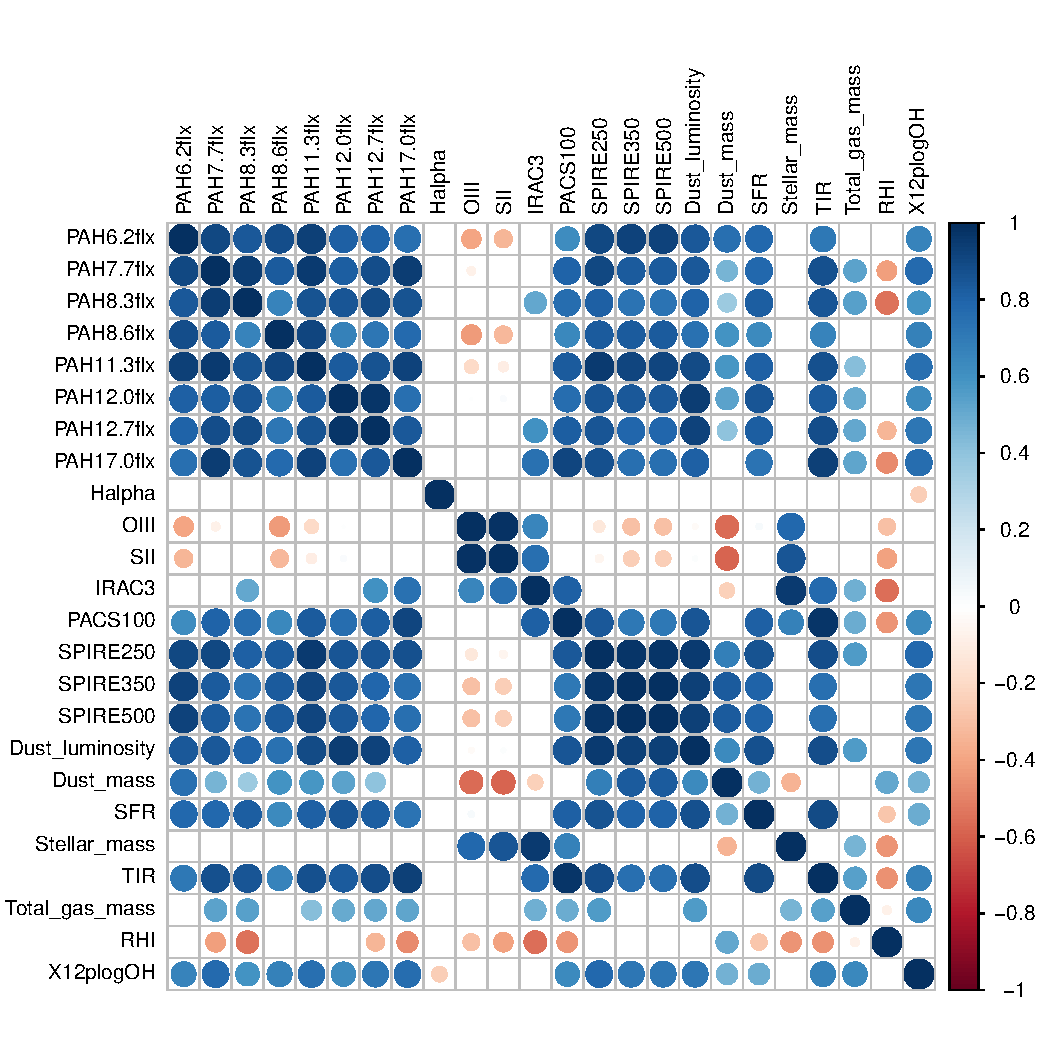
\includegraphics[width=\textwidth]{../image_paper3/images0.01/cor_plots/M31_all_derived_ones_core_plot_for_paper.pdf}
            \caption{Pearson correlation coefficients with a confidence level of 95 per cent for all data from M31. The colours and circle sizes show the Pearson correlation coefficients where large blue circles are 1, which means highly correlated, and large red circles are $-1$, which means highly anti-correlated quantities. The boxes with non-significant correlations were left empty.}
            \label{fig: cor_all}
        \end{figure*}
 
%----------------------------------------------------------------------------------------
%----------------------------------------------------------------------------------------
%----------------------------------------------------------------------------------------
%Result Part 1: 1D SOMs
%----------------------------------------------------------------------------------------
%----------------------------------------------------------------------------------------
%----------------------------------------------------------------------------------------
\section{One dimensional self-organizing maps}
    \label{Sec: 1d_cluster}
%Why 1D maps are useful
    The purpose of  exploring the M31 data with 1D maps is to monitor the general behaviour of the data. 
    One-dimensional SOMs can have the minimum number of clusters, $1\times2$, up to the highest number of clusters possible (infinity).
    In a small sample like ours, smaller grid SOMs are very useful to find correlations that cannot be found without  clustering the data.
    On the other hand, larger grid 1D SOMs are a helpful tool to get quick insight into the data.

    \subsection{Clustering M31 data}%I am not sure about it

        In order to monitor how the data behave, we created SOMs with two to fourteen neurons (Fig.~\ref{fig: M31_nets_1d}).
        The $1\times2$ network (Fig.~\ref{fig: M31_net_1by2}) shows how the M31 data can be divided into two broad categories.
        The $1\times14$ network (Fig.~\ref{fig: M31_net_1by14}) is the first network in which all the regions in M31 are completely separated.
        Since in the higher network sizes, regions have more space to be separated based on their differences, in going from the $1\times2$ to the $1\times14$ network the distance between M31 regions increases, until they are completely separated. 
        
      Fig.~\ref{fig: M31_net_1by2} shows that by forcing the regions in the M31 to be divided into two groups, regions 1, 2, 9 and 10 (shown in Fig.~\ref{fig: regions in m31}) occupy one neuron and the other regions occupy the other one.
        The medium grey colour between two neurons indicates that there are some similarities between two groups, but they are not very similar. 
        By increasing the size of the neurons to three, in Fig.~\ref{fig: M31_net_1by3}, we can see that region 2 separates itself from the other regions and occupies the middle neuron.
        The white colour between two left neurons suggests that the regions which occupy these neurons are very similar to each other, while the black colour between the two right neurons indicates otherwise.
        
        %%%Talking about four right regions
        \cite{Dim15} showed that regions 1, 2, 9, and 10 have higher PAH fluxes compared to other regions (Fig. 5 in \citealt{Dim15}). 
        %Regions 1, 2, and 9 are in the 10~Kpc ring and region 10 is located in the bulge of M31; however, regions 3 to 8 are located slightly out of the inner ring or the 10~kpc one.
        These regions also have relatively high intensities in all the mid-infrared and far-infrared bands and have high dust luminosity and dust mass.
        The higher values for these quantities could be the reason that these 4 regions become separated from the others in the $1\times2$ network.
        Regions 1 and 9 are in the 10~kpc ring, region 2 is slightly out of the 10~kpc ring and region 10 is in the bulge of M31; however, regions 3 to 8 are located out of the inner ring or the 10~kpc ring (Fig.~\ref{fig: regions in m31}).   
        The differences in their positions might be the reason for regions 1, 2, 9 and 10 having higher values in some quantities than the others. 
        Similarities with regions 3 to 8 in the other input values (e.g. SFR) causes regions 1, 2, and 9 to gradually move towards other the regions and away from region 10 in the higher grid SOMs.
       % Therefore, in 1D networks with 14 neurons or higher, regions 1, 2, and 9 completely are separated from region 10, and show more similarity to other regions than to the region 10.
        
        %%% Repeated from the other paragraphs
        %%%Talking about 6 left regions
        %In both Figs.~\ref{fig: M31_net_1by2} and~\ref{fig: M31_net_1by3} the most left neuron is occupied with regions 3 to 8. 
        %These regions all are located outside the inner or 10~kpc rings (See fig.~\ref{fig: regions in m31}).
        %Since the locations of these regions have similar physical properties, they occupy a same neurons in a smaller SOMs.
        %As it can be seen in the $1\times3$ SOM (Fig.~\ref{fig: M31_net_1by3}), the region 2 is moved to the middle neurons.
       % The fact that this region is slightly out of the 10~kpc ring makes region 2 to be the first region to move towards the neurons that occupied with regions 3 to 8. 
       % In the $1\times14$ SOM (Fig.~\ref{fig: M31_net_1by14}), although all the regions were separated, but the colour between regions 10 to the other regions become completely dark.
       % This dark colour indicates that region 10 is absolutely different, which considering the fact that it is the only regions in the bulge of the galaxy, we expected to see such a distance between this regions and the others.
        
    \begin{figure}
    \begin{subfigure}[b]{0.5\textwidth}
        \centering
        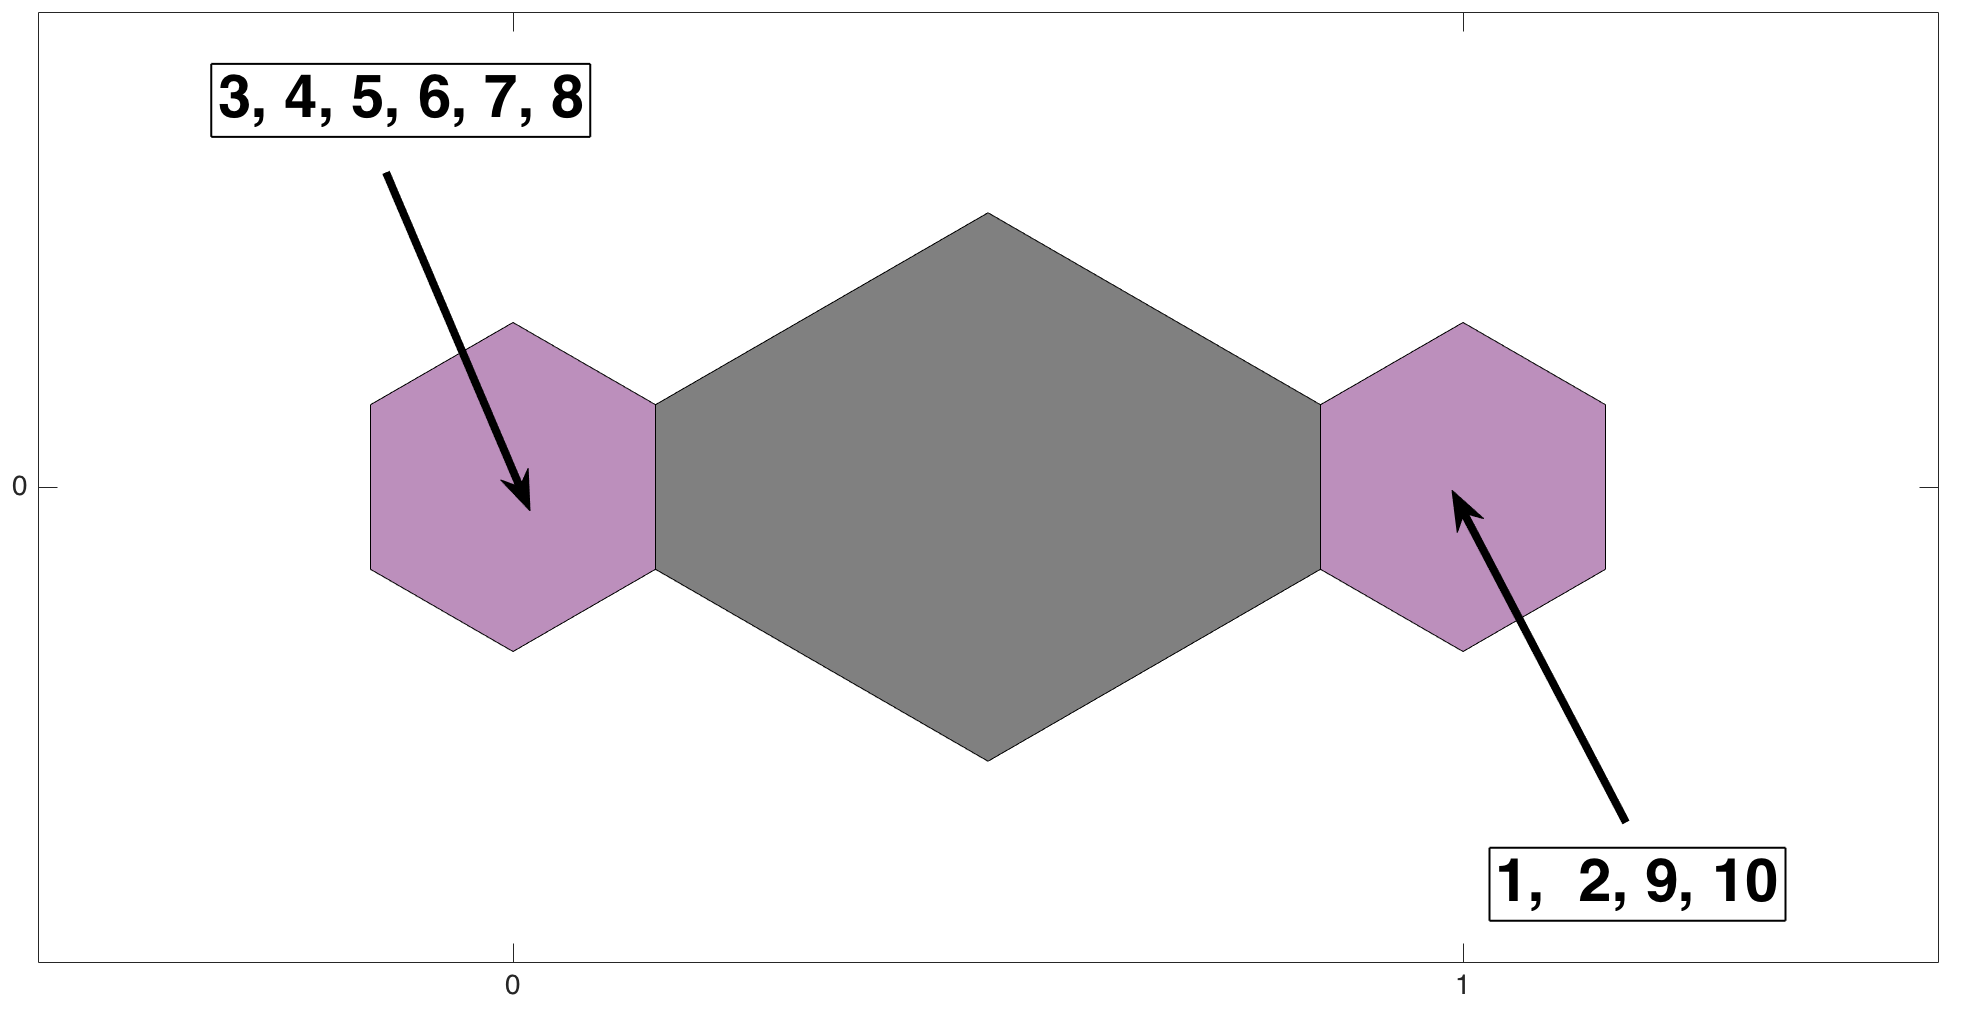
\includegraphics[width=\textwidth]{../image_paper3/images0.01/M31/1D/combine_1D_1by2_all.png}
        \caption{$1\times2$~network}
    \label{fig: M31_net_1by2}
    \end{subfigure}
    \hfill
    \begin{subfigure}[b]{0.5\textwidth}
        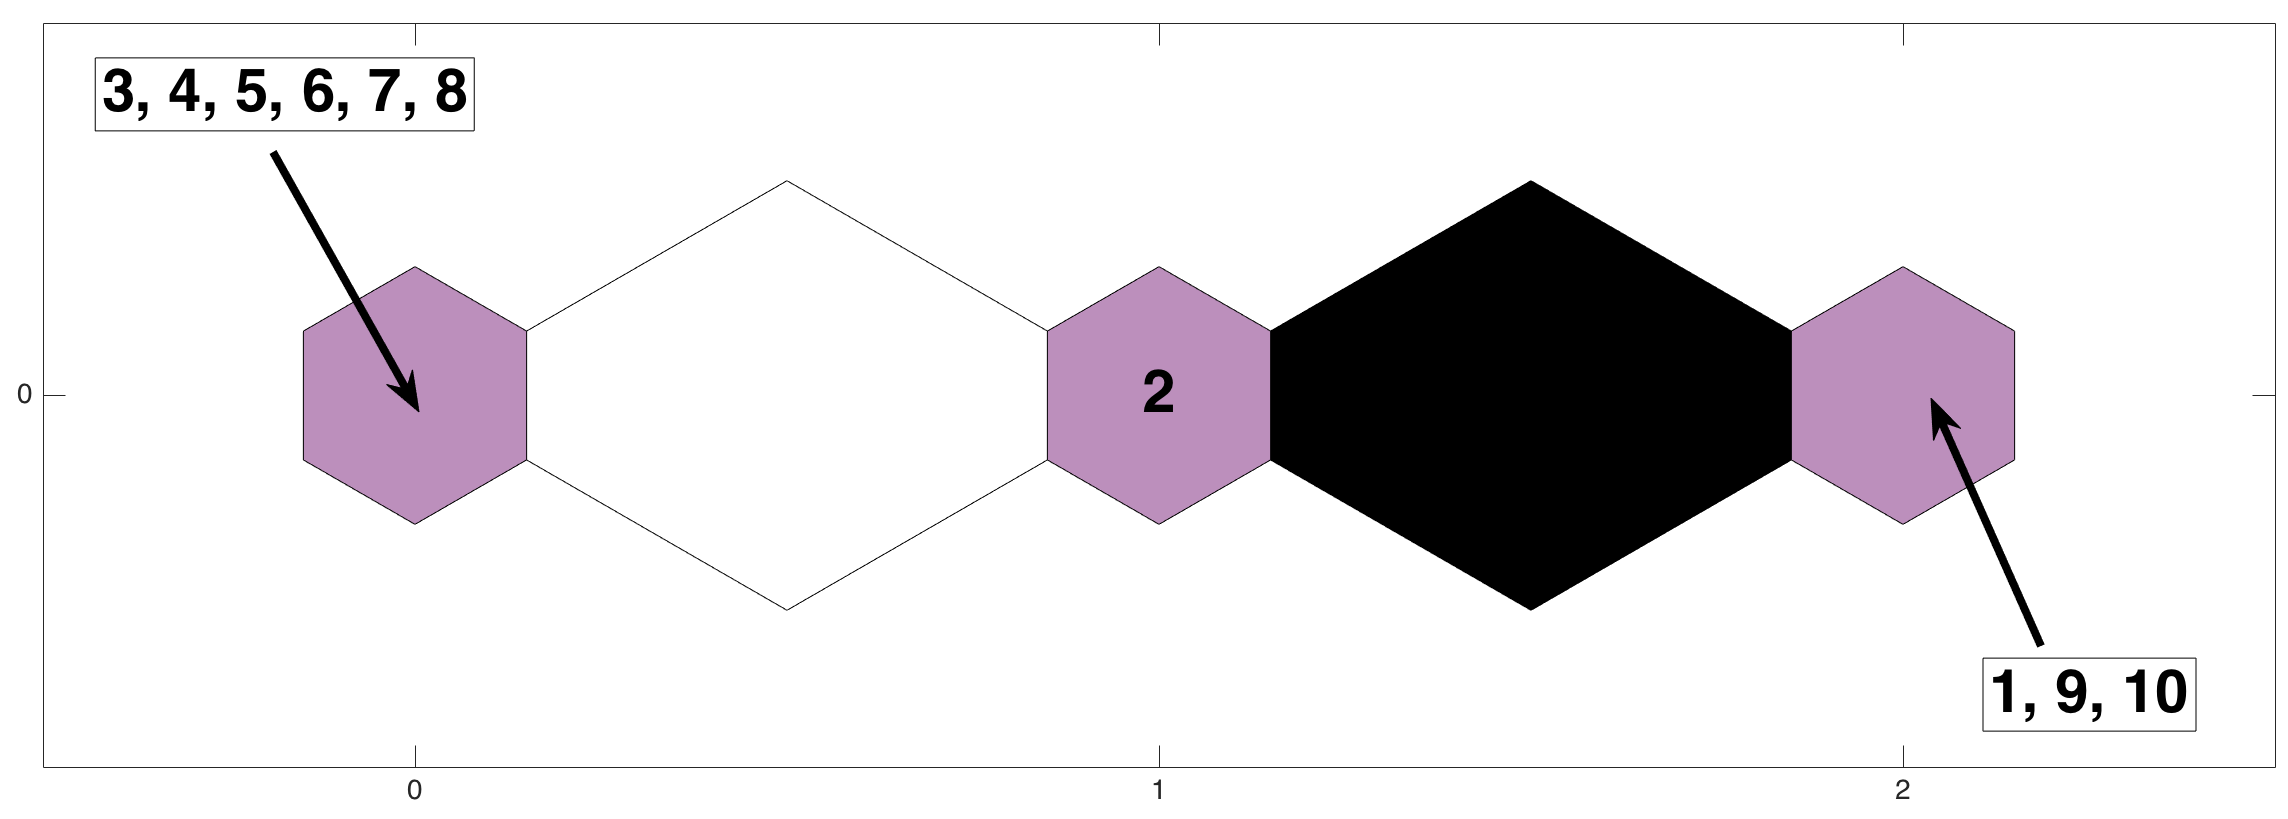
\includegraphics[width=\textwidth]{../image_paper3/images0.01/M31/1D/combine_1D_1by3_all.png}
         \caption{$1\times3$~network}
        \label{fig: M31_net_1by3}
    \end{subfigure}
    \hfill
    \begin{subfigure}[b]{0.5\textwidth}
        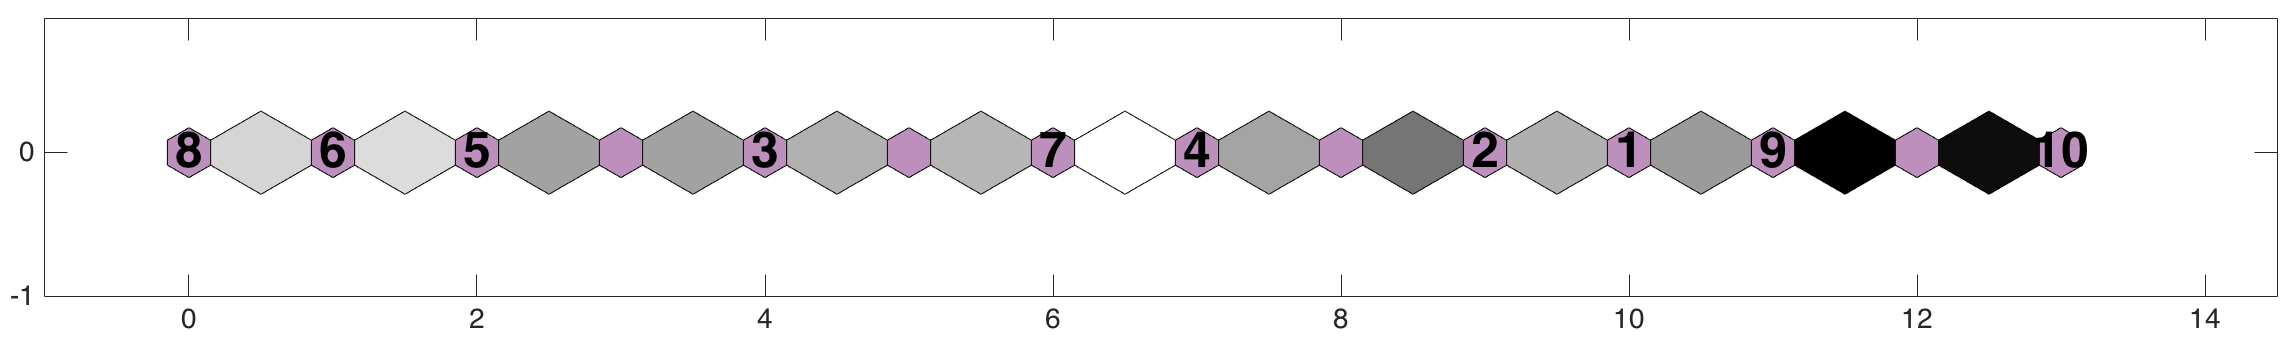
\includegraphics[width=\textwidth]{../image_paper3/images0.01/M31/1D/combine_1D_1by14_all.png}
        \caption{$1\times14$~network}
        \label{fig: M31_net_1by14}
    \end{subfigure}
   \caption{SOM of the M31 data from $1\times2$, $1\times3$~and $1\times14$~grids. The axes show the position of the neurons. The purple hexagonal shapes represent the neurons. The grey scale colours show the differences between the weights of the neurons, with white as the minimum difference and black as the maximum. The numbers in the plot show the M31 regions located in each neuron.}
   \label{fig: M31_nets_1d}
    \end{figure}
    
% \end{figure}
%         \begin{figure}
%             \subfloat[$1\times2$~network\label{fig: M31_net_1by2}]{
%              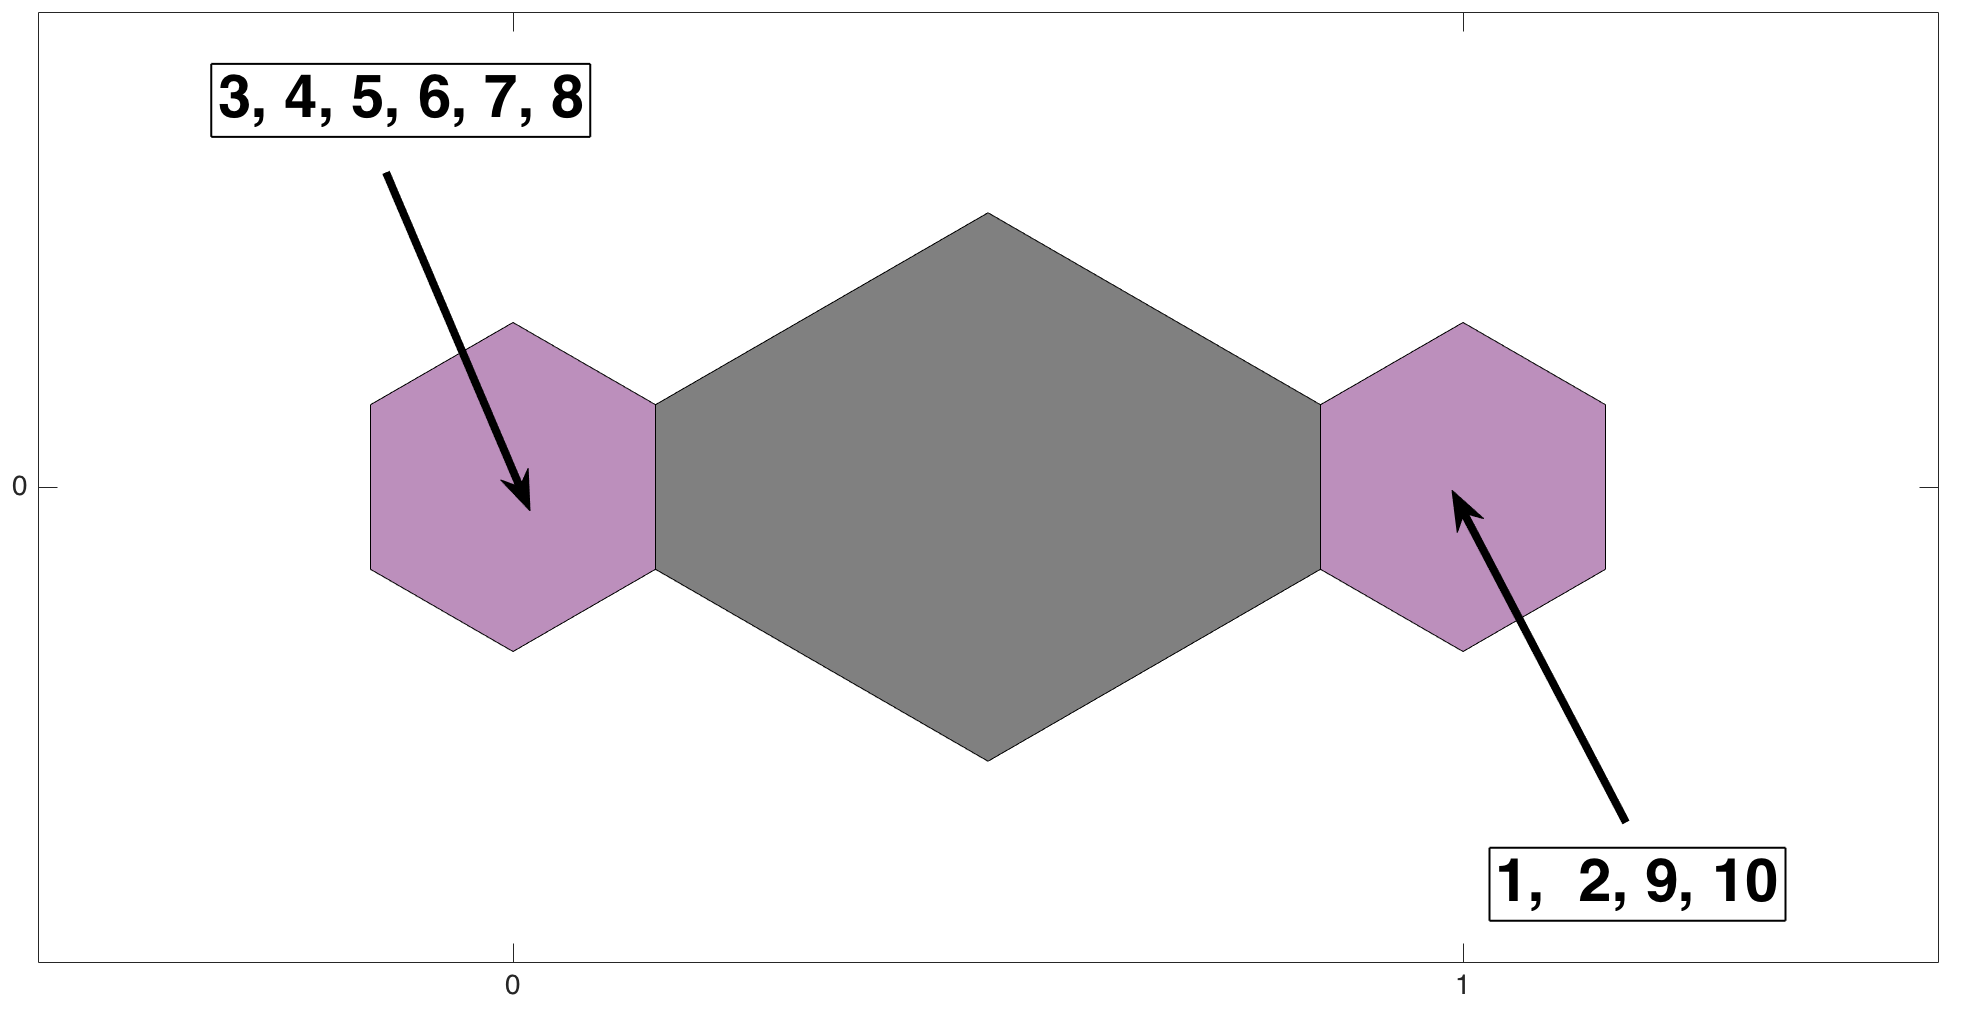
\includegraphics[width=0.5\textwidth]{../image_paper3/images0.01/M31/1D/combine_1D_1by2_all.png}
%              }
%             \hfill
%             \subfloat[$1\times3$~network\label{fig: M31_net_1by3}]{
%             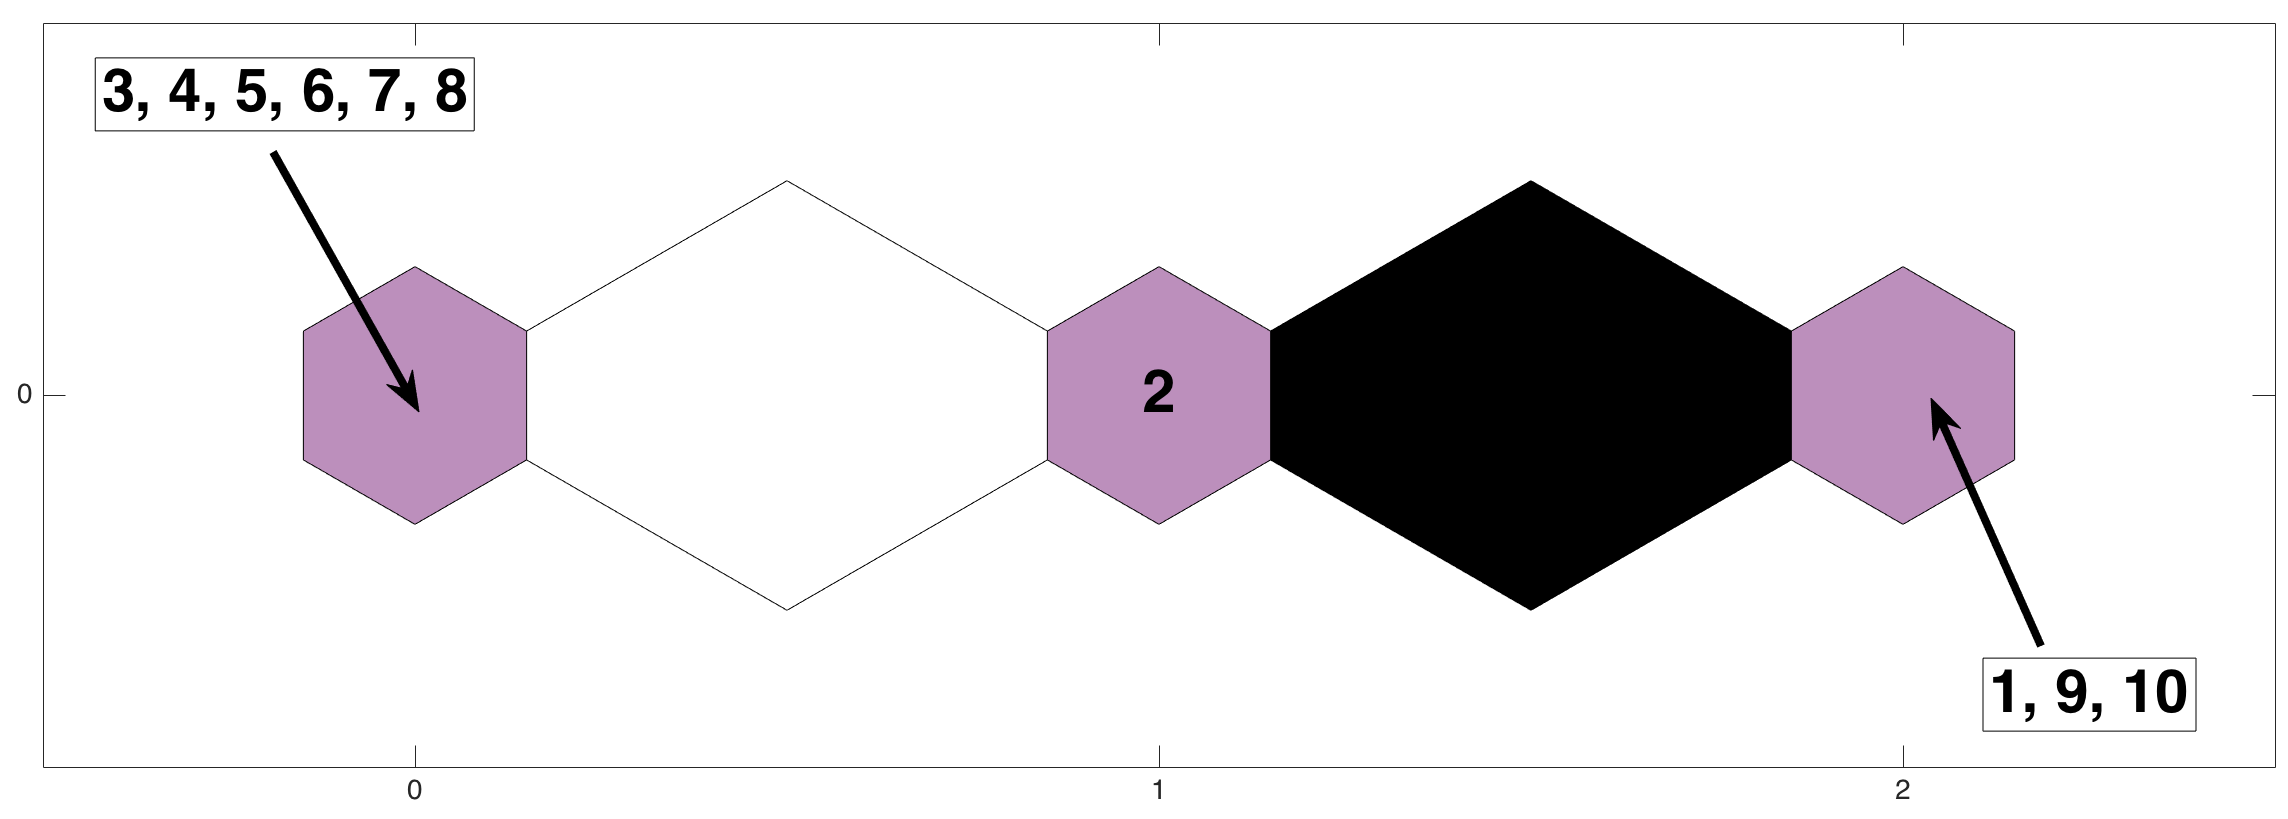
\includegraphics[width=0.5\textwidth]{../image_paper3/images0.01/M31/1D/combine_1D_1by3_all.png}
%              }
%              \hfill
%             \subfloat[$1\times14$~network\label{fig: M31_net_1by14}]{
%              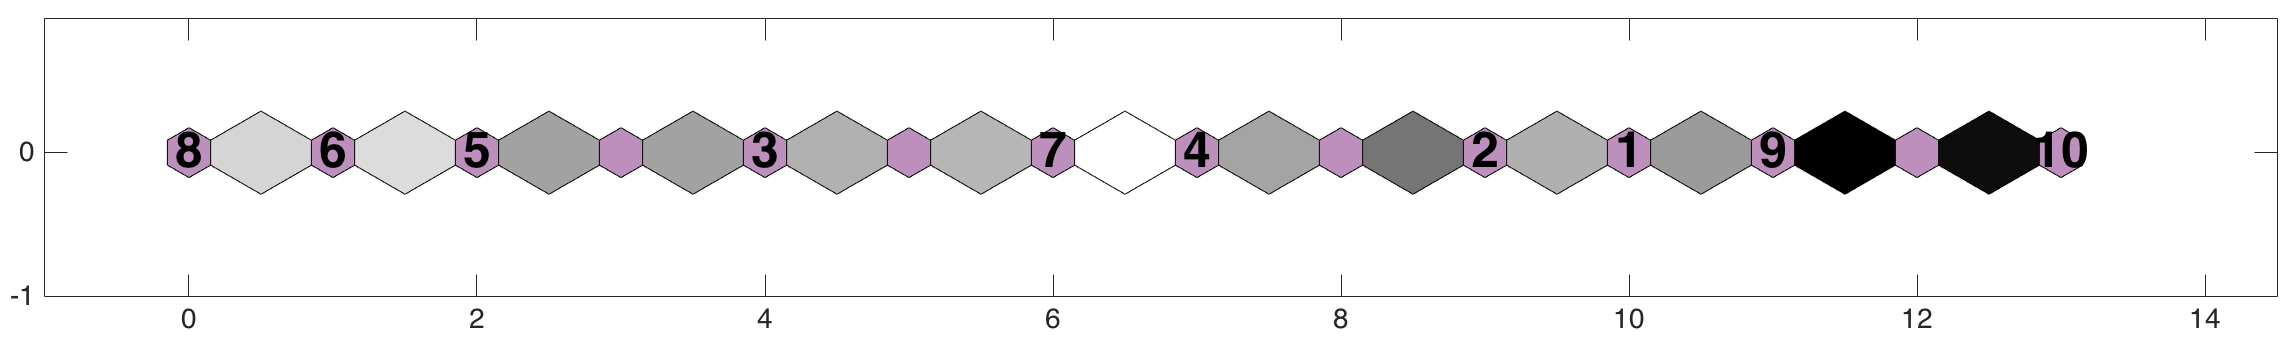
\includegraphics[width=0.5\textwidth]{../image_paper3/images0.01/M31/1D/combine_1D_1by14_all.png}
%              }
%              %%% What should I do with this one! It doesn't look good visually
%             \caption{SOM of the M31 data from $1\times2$, $1\times3$~and $1\times14$~grids. The axes show the position of the neurons. The purple hexagonal shapes represent the neurons. The grey scale colours show the differences between weight of the neurons, with white as the minimum difference and black as the maximum. The numbers in the plot show the M31 regions located in each neuron.}
%             \label{fig: M31_nets_1d}
%         \end{figure}
        
        
        %%Network 1by14
        The network with 14 neurons, in Fig.~\ref{fig: M31_net_1by14}, is the first network that has no neuron occupied by more than one M31 region.
        In a larger-grid SOM, the network pays more attention to smaller details and differences in the input data.
        Since at least 14 neurons are needed to separate all 10 regions in M31, we can conclude that some of the regions have very small differences.
        Regions that are located in similar areas in M31, like regions 7 and 4 (see Fig.~\ref{fig: regions in m31}), are most likely to have more similarities to each other. %%present? show? represent? have?
        In Fig.~\ref{fig: M31_net_1by14}, the right-most neuron is occupied by region 10.
        Two black colours between this region and the others indicate the large differences between this neuron and the others.
       Region 10 is located in the bulge of M31, and is separated from other regions, which are mostly located around the inner or outer rings.
       The SOM shows that this region has completely different input values than the others.
       Most of the input values for region 10 are much higher than the other regions, which is the main reason for its isolation.
        Region 8 occupies the right-most neuron in this network, suggesting that this region has the most differences from region 10.
        
        
    \subsection{Inside the 2 neuron network}
    
        \label{sec: inside_the_2_neurons}
        Using self-organizing maps, we can identify hidden subgroups in our samples. 
        Each of these subgroups were separated from each other for a reason.
        This reason can vary from having higher values in some specific properties, as discussed in Sec.~\ref{Sec: 1d_cluster}, to some unknown correlations between data that cannot be seen in other groups or in the galaxy as a whole.
        To investigate the latter, we show in Fig.~\ref{fig: cor_cluster1} the Pearson correlation coefficients for the inputs from regions 3 to 8, which were clustered together in the $1\times2$ and $1\times3$ networks (see Figs.~\ref{fig: M31_net_1by2} and ~\ref{fig: M31_net_1by3}).
        
        \begin{figure*}
        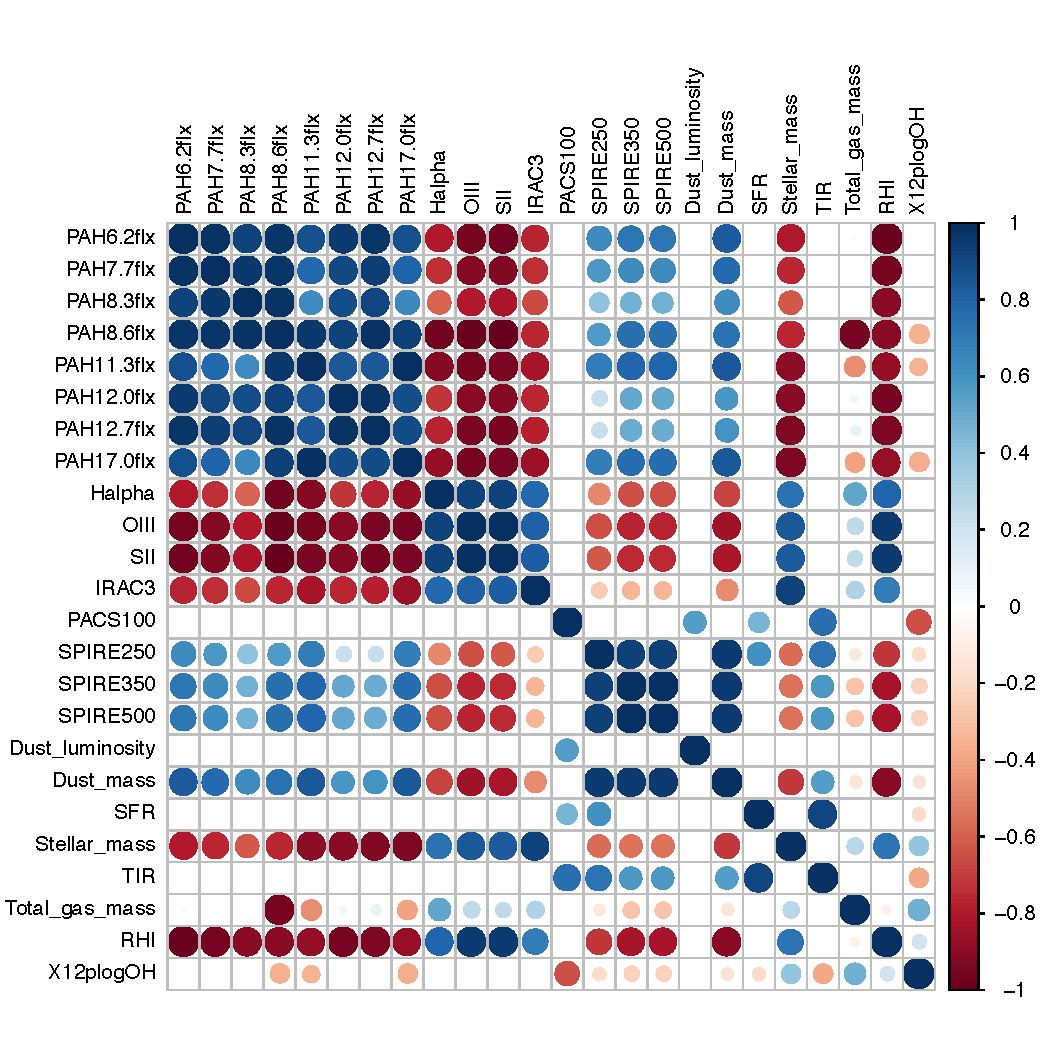
\includegraphics[width=\textwidth]{../image_paper3/images0.01/cor_plots/M31_derived_3_to_8_core_plot_for_paper.pdf}
        \caption{Same as Fig.~\ref{fig: cor_all}, but here we used data from regions grouped in the left sides of Figs.~\ref{fig: M31_net_1by2} and ~\ref{fig: M31_net_1by3}. }
          \label{fig: cor_cluster1}
        \end{figure*}
        
        %%% what regions' version shows and how it compares with the other one:
        In Fig.~\ref{fig: cor_all}, which shows the Pearson correlation coefficients from data in all 10 regions, all the PAH features are highly correlated with each other. 
        Also, there are very strong correlations between all the PAH features and PACS~100~$\mu$m, SPIRE 250 to 500~$\mu$m~emission, L$_{\mathrm dust}$, L$_{\mathrm TIR}$, SFR, and metallicity.
        However, in Fig.~\ref{fig: cor_cluster1}, the 12.0 and 12.7~$\mu$m~PAH fluxes do not show any significant or strong correlation with PAH fluxes at other wavelengths, or with most of the other quantities.
        The only exceptions are the strong correlations between PAH flux at 12~$\mu$m and L$_{\mathrm dust}$, and between the 12 and 12.7~$\mu$m PAH fluxes.
        Since there are only 6 regions in this cluster, even one outlier in the data may cause the correlation coefficient to become insignificant.
        If we ignore the outlier values, the correlations between 12.0 and 12.7~$\mu$m~PAH fluxes and the other quantities reappear. 
        For example, region 8 breaks correlations between 12.0~$\mu$m and 6.2, 7.7, and 8.3~$\mu$m.
        This region could be part of scatter for these correlations, but with 6 regions in the dataset it is hard to have a firm conclusion.
        
        For the PAH fluxes except 12.0 and 12.7~$\mu$m in Fig.~\ref{fig: cor_cluster1}, there are no significant correlations with PACS~100~$\mu$m, L$_{\mathrm dust}$, L$_{\mathrm TIR}$, SFR, or metallicity.
        These PAH fluxes correlate with the SPIRE emission, but to a lesser extent than for the data from all regions.
        Correlations between PAH features and SFR, and L$_{\mathrm TIR}$ are well-studied~\citep[e.g.][]{Tielens08,Peeters04}. 
        Many groups have used PAH features as a tracer of SFR by finding correlations between 
        PAH emission and SFR derived from extinction-corrected \halpha~\citep[e.g.][]{Shipley16,Khramtsova13,Calzetti07}.
        These correlations are seen in Fig.~\ref{fig: cor_all}, when we considered the data from all regions, but not in Fig.~\ref{fig: cor_cluster1} when considering the clustered data.
        Further analyses show that the absence of correlations between PAH fluxes and SFR is because of one outlier: Region 6. 
        When we disregard this region, high correlations between 6.2 to 11.3~$\mu$m~PAHs and SFR (and L$_{\mathrm TIR}$) reappear.
        
        Strong anti-correlations between 6.2 to 11.3~$\mu$m~main PAH features and RHI, stellar mass, \halpha, \sii, \oiii, and IRAC~5.6~$\mu$m~emission in Fig.~\ref{fig: cor_cluster1} were not seen in Fig.~\ref{fig: cor_all}.
        Anti-correlations between PAH features and the \halpha, \sii, and \oiii~emission could be the result of one of the following. 
        First, the optical data are not corrected for dust extinction.
        The PAH features correlate with the amount of dust while \halpha~emission anti-correlates with amount of dust due to extinction \citep{Calzetti94}.
        Therefore, higher PAH fluxes imply higher dust abundance and less \halpha~emission, and the same for \sii~and \oiii~emission.
        Second, is the possible effect of observing apertures.
        If the observed regions are located near the edge of \hii~regions we would expect to see more PAH and less \halpha~emission. %%% reference? PB: I will try to find one.
        The anti-correlations between 6.2 to 11.3~$\mu$m~PAH features and RHI have been seen in other studies, as well~\citep[e.g.][]{Dim15, Gordon08, Wu06}.
        \cite{Wu06} suggested these anti-correlations could be the result of PAH destruction due to a high amount of harder radiation (thus higher RHI).
        On the other hand, \cite{Gordon08} argued that the harder radiation could make the photodissociation regions (PDRs) smaller.
        The PAH features are mostly coming from the PDRs that are surrounded by \hii~regions, and the PAH features' underlying continuum emission is from the \hii~regions.
        Therefore, the lower flux of the PAH features could be the result of the smaller size of PDRs.
        The later reason, which could also describe the anti-correlation between PAH features and \halpha~emission, seems to be the more probable one. 
        
        The strong anti-correlation between PAHs and stellar mass suggests that, despite the general assumption that one of the main source of heating PAHs is stellar emission~\citep[e.g.][]{Jones15,Lu14,Calapa14,Bendo08,Haas02}, a higher stellar mass decreases PAH emission.
        In observations of M33,~\cite{Calapa14} showed that the 8/250~$\mu$m luminosity ratio correlates with 3.6~$\mu$m emission, which translates to stellar mass, and concluded that the PAH emission traces the old stellar population.
        In Fig.~\ref{fig: cor_cluster1}, we see a weak anti-correlation between SPIRE 250~$\mu$m emission and the stellar mass.
        We see no correlation between 8/250~$\mu$m luminosity and stellar mass, either in clustered data or in all 10 regions.
      %  The results from~\cite{Calapa14} were based on data from the whole galaxy and has a relatively high scatter.
      %It is possible that all the 10 regions in M31 simply aligned with the scatter of the correlation. Further analysis on M31 data is required to see weather the anti-correlation in this regions is extended to whole galaxy or it is only for these 6 regions.
        
        Some studies have indicated that strong stellar emission could lead to destruction of PAHs ~\citep[e.g.][]{Clayton03,Seok14}.
        To test whether anti-correlation between stellar mass and PAH emission is the result of the destruction of PAHs in high stellar mass regions, or that high stellar mass obscures PAH emission, we compared PAH abundance with stellar mass for the clustered regions.
        The ratio of 8/24~$\mu$m emission, which can be considered as a proxy for PAH abundances~\citep[e.g.][]{Sandstrom10,Khramtsova13}, does not anti-correlate with stellar mass for either the clustered data or all 10 regions.
        Therefore, we conclude that in our sample,  stellar mass does not cause the destruction of PAHs.
        
        The anti-correlation between stellar mass and PAHs could be result of the position of the regions in M31.
        Regions 5, 6, and 8 are located on the stellar disk of the galaxy and have relatively high stellar mass and low PAHs. 
        According to~\cite{Dim15}, regions 5 and 8 are the only two regions in our sample that do not include an \hii~region, which could be the reason of low PAHs for these regions.
        Regions 4 and 7 have similar quantities for both stellar mass and PAHs and region 3 has high PAHs and low stellar mass.
        Without data from more regions in M31, we cannot confidently say that higher stellar mass decreases PAH fluxes.
        %% Sahar: Can we have higher PAHs absorbes stellar mass and thats why we see the anti-correlation?!!!
        
       % On the other hand, if we divide SFR by stellar mass, which give us specific star formation rate (sSFR), we see strong correlation between sSFR and 6.2 to 11.3~$\mu$m fluxes for clustered regions,
        
        
       Regardless of the fact that some of the (anti)-correlations in Fig.~\ref{fig: cor_cluster1} might have physical meaning, we have to mention that we only used 6 regions to calculate these correlation coefficients.
       The number of data points is not high enough to yield a strong conclusion about PAH properties in M31.
        However, we can conclude that since the correlation coefficients derived from the clustered data (Fig.~\ref{fig: cor_cluster1}) differ from the correlation coefficients derived from the data from the all regions (Fig.~\ref{fig: cor_all}), the SOM separated a hidden cluster of the data which has different properties.
        
        
        
 %----------------------------------------------------------------------------------------
%----------------------------------------------------------------------------------------
%----------------------------------------------------------------------------------------
%Result Part 2: 2D SOMs
%----------------------------------------------------------------------------------------
%----------------------------------------------------------------------------------------
%----------------------------------------------------------------------------------------
 \section{Two dimensional self-organizing maps}
 \label{sec: 2d_cluster}
    Although 1D networks are helpful to give a general idea about the data, neurons in 1D maps have a maximum of two neighbours, which can limit the usefulness of the results.
    In 2D networks, each neuron has two to six neighbours, which allows them to capture a complete picture of the complicated relations in the input data.
    Accordingly, we created $10\times10$ 2D networks to study the data in detail.
    As mentioned in previous sections, the size of SOMs are arbitrary and must be decided by users based on their goals for use of the SOM.
    
    In this section we chose $10\times10$ size despite knowing, from the size of our input data, that most of the neurons would be empty.
    Using 2D networks, we are mostly interested in the ability of the SOMs to show the underlying structure of the data rather than its clustering features.
    Fig.~\ref{fig: all_derived_ones} shows the 2D SOM of the M31 data.
    Similar to Fig.~\ref{fig: M31_net_1by14}, all the 10 regions are completely separated from each other in Fig.~\ref{fig: all_derived_ones}.
    \import{../image_paper3/text_files/image_texts/}{all.tex}
    
    Regions 4 and 7 are in the top left of Fig.~\ref{fig: all_derived_ones} with a very bright colour between their neurons, indicating that these two regions are very similar.
    Considering the position of these two regions in M31 (both right on the edge of the star forming rings in the galaxy), similarity of these two regions was predictable.
    The position of region 3 on the SOM is close to the position of regions 4 and 7, but with a darker colour between the nodes. 
    In Fig.~\ref{fig: regions in m31} it is clear that this region in M31 is physically closer to regions 4 and 7 than to any other region, but it is on the outer side of the star forming ring.
    Regions 5 and 6 are in the second neighbourhood on the SOM, with a medium gray colour between them.
    These two regions are physically located around the inner ring of the galaxy.
    Regions 8 and 6 are both in the inner ring of M31, but region 6's location has more star formation, which could be the main reason for their relative distance in the SOM in Fig.~\ref{fig: all_derived_ones}. 
    
    Regions 1 and 9 are close to each other, and in the same side of the star forming ring. 
    However, region 1 is in an area of the galaxy with less diffuse \halpha~emission than region 9, which might be the reason for their distances in SOM.
    Region 2 is more distant from other regions in the galaxy and placed in the star forming ring.
    However, similar to regions 1 and 4, region 2 is located in an area of the galaxy with less diffuse \halpha~emission.
    Therefore, the place of region 2 in the SOM tends towards regions 1 and 4. 
    Region 10 is in the bulge of the galaxy, and its position on the SOM is isolated from all the other regions by a strip of a dark colours. 
    
    In order to analyse effects of any input data on the final SOM, in the following we create SOMs from various subsets of data.
    We compare results of the subsets with one another and with the SOM created from all data in Fig.~\ref{fig: all_derived_ones}.

    \subsection{Subsets}
    \label{sec: subsets}
            For analysing subsets, we created SOMs by using only PAH data, as well as using all data except the PAHs (Fig.~\ref{fig: PAHS_or_not_PAHs}).
             \import{../image_paper3/text_files/image_texts/}{PAHS_or_not_PAHs.tex}
            Comparing the SOM from all data in Fig.~\ref{fig: all_derived_ones} with the SOMs in Fig.~\ref{fig: PAHS_or_not_PAHs} shows that the general position of regions in those networks are the same. 
            Region 10 is in one corner of all three networks.
            However, in Fig.~\ref{fig: all_derived_ones} and Fig.~\ref{fig: wt_pahs}, region 10 is isolated from the other regions, while in Fig.~\ref{fig: only_pahs}, region 10 is much less isolated and only shows complete dissimilarity with region 8.
            Regions 9 and 10 are totally isolated in the SOMs in Fig.~\ref{fig: wt_pahs}, but in Fig.~\ref{fig: only_pahs}, they are more similar to other regions.
            In both SOMs in Fig.~\ref{fig: PAHS_or_not_PAHs}, there are dissimilarities between regions in M31 but in Fig.~\ref{fig: wt_pahs}, the colours are much darker than the ones in Fig.~\ref{fig: only_pahs}.
            This indicates that there is more similarity between the PAH features over all 10 regions than between the other input data.
            
            We increased the dimension of input data in Fig.~\ref{fig: only_pahs} (PAH only data) gradually, by adding other quantities to the input data. 
            The order in which data were added is the same as the order in Fig.~\ref{fig: cor_all}, i.e. the SOM in Fig~\ref{fig: col3and11_dist} was created from PAH and H$\alpha$ emission as input data, the SOM in Fig~\ref{fig: col3and12_dist} created from PAHs, H$\alpha$ emission and \sii~ continuum, and so on. 
            \import{../image_paper3/text_files/image_texts/}{col3byall.tex}
            
            The SOM algorithm assigns a random weight to each network that causes the overall position of regions in networks (even with the same input data) to change in each run of the algorithm.
            However, the position of each region relative to other regions changes dramatically only when the new sets of input data are given to the algorithm (assuming all the initial values for the run are unchanged).
            In all SOMs in Fig~\ref{fig: inc_D_col3s}, region 10 is located in the corner of the SOMs, but in  Figs~\ref{fig: col3and11_dist},~\ref{fig: col3and14_dist},~\ref{fig: col3and17_dist},~\ref{fig: col3and21_dist}, and ~\ref{fig: col3and22_dist}, it is placed in the left side of the SOMs and in the others it is in the right side of the networks.
            In our discussion on differences between networks, we do not address the changes in the network due to initialization of the SOM algorithm and only consider the effect of changing the input data.
            
            Comparing Figs.~\ref{fig: col3and11_dist} to ~\ref{fig: col3and25_dist} shows that adding \halpha~emission data to PAH features causes regions 9 and 10 become isolated. 
            Increasing the dimension of the input data makes region 10 more isolated.
            The relative positions of regions 4 and 7 stay the same with increasing the dimensions of the input data. 
            Adding SPIRE 350, 500~$\mu$m emission and L$_{\rm dust}$ does not have any obvious effect on the networks.
            Stellar mass, total gas mass, dust mass and RHI data alternate the distances between neurons effectively, but it seems that adding SFR, L$_{\rm TIR}$ and metallicity data revoke those changes.
            
            We generated other subsets of the data based on the results in Figs~\ref{fig: inc_D_col3s} to further study the effects of the input data on SOMs.
            Subset 1, listed in Tab.~\ref{tab: subset1}, includes all the input data except stellar mass.
            Tab.~\ref{tab: subset5} lists data used in subset 2, which includes all data except that the PAH fluxes are combined into a total PAH flux. 
            For subset 3 ( in Tab.~\ref{tab: subset6}), SPIRE 250 and 500~$\mu$m were removed from subset 2.
            Figs.~\ref{fig: subset1} --~\ref{fig: subset6} show SOMs created by data from subsets 1 to 3, respectively.
            The remaining subsets are discussed in Appendix.~\ref{sec: app_2d_soms_SOMN}.

            The results from Table~\ref{tab: subset1} are shown in Fig.~\ref{fig: subset1}. 
            In this SOM, compared with the SOM from all the data in Fig.~\ref{fig: all_derived_ones}, regions 1 and 9 are closer to region 10. 
            Regions 1 and 9 are the ones with lowest stellar mass values, and region 10 has the highest stellar mass value among those 10 regions. 
            Since the differences in the amount of stellar mass was one of the most distinct differences between these three regions, removing stellar mass from the input data reduced the distance between these regions.
            Regions 5, 6 and 8 have the same relative distance from each other as in Fig.~\ref{fig: all_derived_ones}, but they  are all closer to the position of region 10.
            The distance between regions 2 and 3 is reduced but in the meantime the colour between them became darker.

            \import{../image_paper3/text_files/tables/}{subset1.tex}
            \import{../image_paper3/text_files/image_texts/}{subset1.tex}

            Changing from separate values for each PAH feature to a single value for the total PAHs caused small changes to the SOM map in Fig.~\ref{fig: subset5} compared to the one in Fig.~\ref{fig: all_derived_ones}. 
            The distance between the positions of regions 6 and 8 increased significantly, while the position of region 2 moved closer to the positions of regions 4 and 7.
            The winner neurons for regions 3 and 5 moved towards each other, but the colours between them became much darker. 

            \import{../image_paper3/text_files/tables/}{subset5.tex}
            \import{../image_paper3/text_files/image_texts/}{subset5.tex}

            Fig.~\ref{fig: subset6} shows the SOM generated from data listed in Tab.~\ref{tab: subset6}, which includes all the data from Tab.~\ref{tab: subset5} except for  the SPIRE 250 and 500~$\mu$m emission.
            Although for most of the regions we see the changes in their positions, the colours between neurons changes as well. 
            %Therefore, we can conclude that these changes caused by the differences in the initial assigned weights.
            The distance between the positions of the regions 4 and 2 is increased as are the
            distances between regions 7, 3 and 6.
            In both cases, SPIRE 250 and 500~$\mu$m emission of these regions are similar to one another, and removing these two parameters from the input data moved the positions of the regions further from each other. 
            \import{../image_paper3/text_files/tables/}{subset6.tex}
            \import{../image_paper3/text_files/image_texts/}{subset6.tex}
            
            %Subsets, that some of them  are studied in this section, can be used to learn about the effect of each input on the map as well as they can be used to predict unobserved quantities in the galaxy.
            
            % \subsubsection{Prediction observing data using M31}
        
            %     On SOMs we can see relations between the input data from each region regarding to the other regions.
            %     These relations are shown by colour in SOMs, when white is 100 per cent similarity and black is 0 per cent similarity.
            %     Therefore, we have the probability distribution of quantities of each values given data from other regions.
            %     We can use these probability distribution to estimate missing data for regions. 
                
            %     To demonstrate this conclusion, we assumed the stellar mass value for region 1 is unknown.
            %     Therefore, we need a SOM that are generated from all the inputs data for all regions except stellar mass (e.g subset 1 in Fig.~\ref{fig: subset1}).
            %     \import{../image_paper3/text_files/image_texts/}{sim_subset1.tex}
            %     We found the shortest path between region 1 and the other regions and measure their relative similarity ($p_j$).
            %     Assuming the maximum similarity is 100 per cent between two neurons (white colour), we multiply the similarity values along the shortest path between two regions to find $p_j$ between region 1 and the other regions (Fig.~\ref{fig: sim_subset1}).
            %     In both Figs.~\ref{fig: subset1} and ~\ref{fig: sim_subset1} are clear that region 1 shows more similarity to regions 2 and 9 than the others and the most dissimilarity to region 8. 
                
            %     We measured probability of stellar mass given other quantities of the region 1 ($P(m_1\mid \forall_1)$) using Equation~\ref{equ: prob1}.
            %     \begin{equation}
            %     \label{equ: prob1}
            %         P(m_1\mid \forall_1) = \sum_{j=2}^{10}p_j*m_j
            %     \end{equation}
            %     Where $m_1$ is the stellar mass of region 1 and $m_j$ is the stellar mass of region j (any other region).
            %     We estimated the stellar mass to be $\sim1377$~M$\odot$ which is 10 per cent less than the observed values.
            %     This type of the prediction from SOM networks can be used to predict observation values in observational proposals or can be used in pre-phase studies of the big missions such as the James Webb Space Telescope (JWST) and LLST.
                

    \subsection{Testing networks using M101 observations}
    Another application of self-organizing maps made with data from a single galaxy is to apply its trained networks on data from other galaxies to make predictions. %%eh
    To demonstrate this, we generated an SOM using only M31 measurements which were also available for M101 (Fig.~\ref{fig: subset9}a). 
    \cite{Dim15} compared PAHs in M31 with those from H {\sc II} regions in M101, and showed the similarity between PAHs in these two galaxies (for more detail see \cite{Dim15} and \cite{Gordon08}).
    In this SOM, as in the others, region 10 is separated from other regions in M31.
    Regions 7 and 4 are close to each other with very light colours between their neurons, and as in the other SOMs regions 6, 8, and 5 are close to each other, but with a medium dark colour between them.
    \import{../image_paper3/text_files/image_texts/}{subset9.tex}
    
    We applied the SOM created using M31 data in Fig.~\ref{fig: subset9}a to M101 data (Fig.~\ref{fig: subset9}b).
    Region 5 in M31 and region 8 in M101 and regions 6 in M31 and region 2 in M101 occupied neurons with a white colour between them in the network in Fig.~\ref{fig: subset9}, which immediately suggests that these regions have similar properties. 
    Region 2 in M101 is a bright H {\sc II} region located at the end of the one of the M101 spiral arms (see Fig.~\ref{fig: regions in m101}) while
    region 6 in M31 is located near the inner star-forming ring (see Fig.~\ref{fig: regions in m31}).
    Both regions have relatively low PAH emission and a median amount of  SFR compared to other regions in the galaxy, making them very similar.
    
    Region 5 in M31 is in the inner ring of the galaxy and it is one of two regions in M31 that are not an  H {\sc II} region, while
    region 8 in M101 is in a spiral arm of the galaxy.
    Relatively low stellar mass, SFR and SPIRE band emission caused these two regions to be nearby in the map.
    In Sec.~\ref{Sec: 1d_cluster} we showed that regions 3 to 8 in M31 have similar properties; in Fig.~\ref{fig: subset9}b we see that regions 1 to 3 and 5 to 8 in M101 are located near regions 3 to 8 in M101. 
    These regions all have medium or low PAH emission, dust and SFR compared to the remaining regions.
    
    Region 7 in M101 is located in the nucleus of the galaxy and has relatively higher values of the quantities than the other regions.
    This region is located in the top right side of the network in Fig.~\ref{fig: subset9},  close to the location of M31 region 10 in the network.
    Since the bulge of a spiral galaxy has a different environment from its nucleus, region 7 in M101 and region 10 in M31 do not occupy the same neuron in the SOM, and have a medium grey colour between their neurons.

    Region 1 in M101 is also located near the nucleus of M101 (see Fig.~\ref{fig: regions in m101}), but has considerably lower values in all the quantities compared to region 7.
    The lower values for fluxes of the PAH features and moderate amount of the SFR caused this region to be placed between M31 regions 4 and 5 in the network. 
    Fig.~\ref{fig: subset9}b shows that region 4 in M101 is separated from other regions and located between M31 regions 9 and 10.
    \cite{Gordon08} showed that this region is a diffuse nebula in M101, with high PAH emission. 
    This region also shows a high SFR and stellar mass, explaining why the location of M101 region 4 in the SOM is close to that of M31 regions 9 and 10.
    
    Knowing the effects of the different input quantities on the networks from Section~\ref{sec: subsets}, we can have ideas about data entry from other regions/galaxies.
    In this section we showed that we can use networks that are created by data from nearby galaxies, to study the properties of other galaxies in a fast way.
    We should note that, since we normalized data before using them in the networks, we only see relative properties of the regions.
    Therefore, we need data from few regions in the galaxy to use this network and cannot use these networks to learn about properties of a single region in other galaxies.
    
    
%----------------------------------------------------------------------------------------
%----------------------------------------------------------------------------------------
%----------------------------------------------------------------------------------------
%Summery
%----------------------------------------------------------------------------------------
%----------------------------------------------------------------------------------------
%----------------------------------------------------------------------------------------
\section{SUMMARY}
\label{sec: summary}

We present results of studying spatially resolved regions in nearby galaxies using Kohonen self-organizing maps.
Self-organizing maps both cluster data and show relative distance between the clusters. 
We utilized the method to find hidden subgroups in the data as well as finding relations between those groups.

Using smaller-sized self-organizing maps, we found that the M31 data are clustered into two major groups, which led us to correlations that could not have otherwise been seen without clustering.
Six of the regions in M31 create a subgroup with relatively lower mid- and far-infrared emission.
PAH fluxes in these regions are highly anti-correlated with \halpha, \sii, \oiii~and IRAC 5.8~$\mu$m emission, stellar mass and radiation hardness index.
These anti-correlations are insignificant when the full dataset is considered.
The most probable reason for PAHs to anti-correlate with optical emission lines and RHI is a harder radiation field.
This makes the size of \hii~regions bigger and the size of photo-dissociation regions smaller, causing more \halpha~emission and less PAH emission, respectively.

PAHs in clustered data also show an anti-correlation with stellar mass.
We discussed the possibility that higher stellar mass might destroy PAHs;
however, we did not find any correlation between 8/24~$\mu$m emission, as a tracer of PAH abundance, and stellar mass.
Unlike previous studies, we also did not find any correlation between 8/250~$\mu$m emission and stellar mass. 
This result shows that PAHs in the clustered regions in M31 are not heated by the old stellar populations.

In self-organizing maps with larger sizes, networks can be used to illustrate the relations of the regions with one another.
We found the relative similarity between M31 regions by varying the size of the networks.
A one-dimensional network with 14 neurons was needed in order to
separate all 10 regions; some of the regions in M31 (e.g. regions 4 and 7) have very similar properties.
Two-dimensional networks provide us with a more complete picture of the data.
We created various subsets of the input data and generated different networks which helped to show relations between regions in M31 more clearly.
Region 10 always becomes isolated in the networks, except when we  used only PAH data to create a network. %PB: remind the reader where regions 8 and 10 are
In that network region 10 blends more with other regions and only shows differences with the data from region 8.
These results suggest that the PAHs in all 10 regions have almost the same properties.

Applying the SOMs from M31 to observations of M101, we found regions with similar properties in both galaxies placed in close regions in the SOMs.
Using this ability of the SOM, we can predict properties of regions in other nearby galaxies very quickly.
The networks we created used values for 26 quantities from 10 regions in M31, which is not a large sample.
Increasing the dimension of the data and the number of regions would yield more reliable networks.
In future we can apply these networks on data from other nearby galaxies (e.g. M33 and M83) and learn about the properties of regions in those galaxies.

%----------------------------------------------------------------------------------------
%----------------------------------------------------------------------------------------
%----------------------------------------------------------------------------------------
%biblio
%----------------------------------------------------------------------------------------
%----------------------------------------------------------------------------------------
%------------------

\addcontentsline{toc}{section}{Bibliography}
\bibliographystyle{apj.bst}
\bibliography{ref_paper3.bib}